\documentclass{statsoc}

\usepackage[a4paper]{geometry}
\usepackage{graphicx}
\usepackage[textwidth=8em,textsize=small]{todonotes}
\usepackage{amsmath}
\usepackage{amsfonts}
\usepackage{enumerate}
\usepackage{amsmath}
\usepackage{mathrsfs}
\usepackage{color}
\usepackage{amssymb}
\usepackage{tikz-cd} 
\usepackage[export]{adjustbox}
\usepackage{subfig}
\usepackage{booktabs}
\usepackage{algorithm, algcompatible}

\algnewcommand\INPUT{\item[\textbf{Input:}]}%
\algnewcommand\OUTPUT{\item[\textbf{Output:}]}%
\def\cc{\color{blue}}
\usepackage[normalem]{ulem}

\newtheorem{theorem}            {Theorem}[section]
\newtheorem{proposition}        [theorem]{Proposition}

\newcommand{\CC}{\mathbb{C}}
\newcommand{\RR}{\mathbb{R}}
\newcommand{\NN}{\mathbb{N}}
\newcommand{\QQ}{\mathbb{Q}}

\usepackage{natbib}
\bibliographystyle{unsrtnat}
\renewcommand{\bibsection}{}

\title[GuidedSparseKmeans]{Outcome-Guided Sparse K-Means for Disease Subtype Discovery via Integrating Phenotypic Data with High-Dimensional Transcriptomic Data}
\author[]{Group 7: I Hung, Nathan, Paul}
\address{Penn State University}

\begin{document}

\section{Problem Description and Modeling Objective}

The challenge in precision medicine is to identify disease subtypes linked to clinical outcomes, as traditional methods often miss complex connections between biological data and clinical traits, resulting in less effective treatments. This study introduces the GuidedSparseK-means algorithm, which integrates clinical data with high-dimensional omics data to address the need for innovative approaches. The algorithm employs a unified objective function that combines weighted K-means clustering, lasso regularization for gene selection, and the inclusion of a phenotypic variable. By iteratively optimizing this function, GuidedSparseK-means aims to yield statistically robust and clinically relevant subtypes, enhancing the potential for personalized treatment strategies.

\section{Data Description}

The study utilizes high-dimensional gene expression data and clinical phenotypic data from modern epidemiological cohorts, specifically focusing on transcriptomic datasets related to breast cancer and Alzheimer disease.

Gene expression data is used to understand how genes are active in different conditions, such as in healthy versus diseased tissues. By measuring which genes are turned on or off, we can learn about the biological processes happening in a cell.~\citep{emilsson2008genetics} This data helps identify genes involved in diseases like breast cancer and Alzheimer disease, as used in the study~\citep{meng2022outcome}.

The METABRIC breast cancer gene expression data~\citep{curtis2012genomic} included samples from tumor banks in the United Kingdom and Canada. It contains gene expression profile of 20,603 genes and 2,501 subjects (see Fig.~\ref{fig:metabric_expr} for details). It also contains various clinical data for every sample, particularly the Nottingham prognostic index (NPI); Estrogen receptor status (ER); HER2 receptor status (HER2); and overall survival (see Fig.~\ref{fig:metabric_data} for details).

Breast cancer is often tested for three key factors: NPI, ER, and HER2 status, which help guide treatment~\citep{haybittle1982prognostic, jensen1973estrogen, di1987erb}. NPI is a score based on the size of the tumor, the grade of the cancer cells, and how many lymph nodes are affected, helping predict how aggressive the cancer is and how likely it is to spread. ER status checks if the cancer cells have receptors for estrogen, a hormone that can fuel cancer growth. If the cancer is ER-positive, it means estrogen helps the cancer grow, and treatments that block estrogen, like hormone therapy, can be effective. HER2 is a protein that helps cancer cells grow, and if the cancer is HER2-positive, it means the cancer cells have too much of this protein. Targeted therapies like Herceptin can help treat HER2-positive cancers. Together, these tests help doctors determine the best treatment plan for each patient.

\begin{figure}[h!]
    \centering
    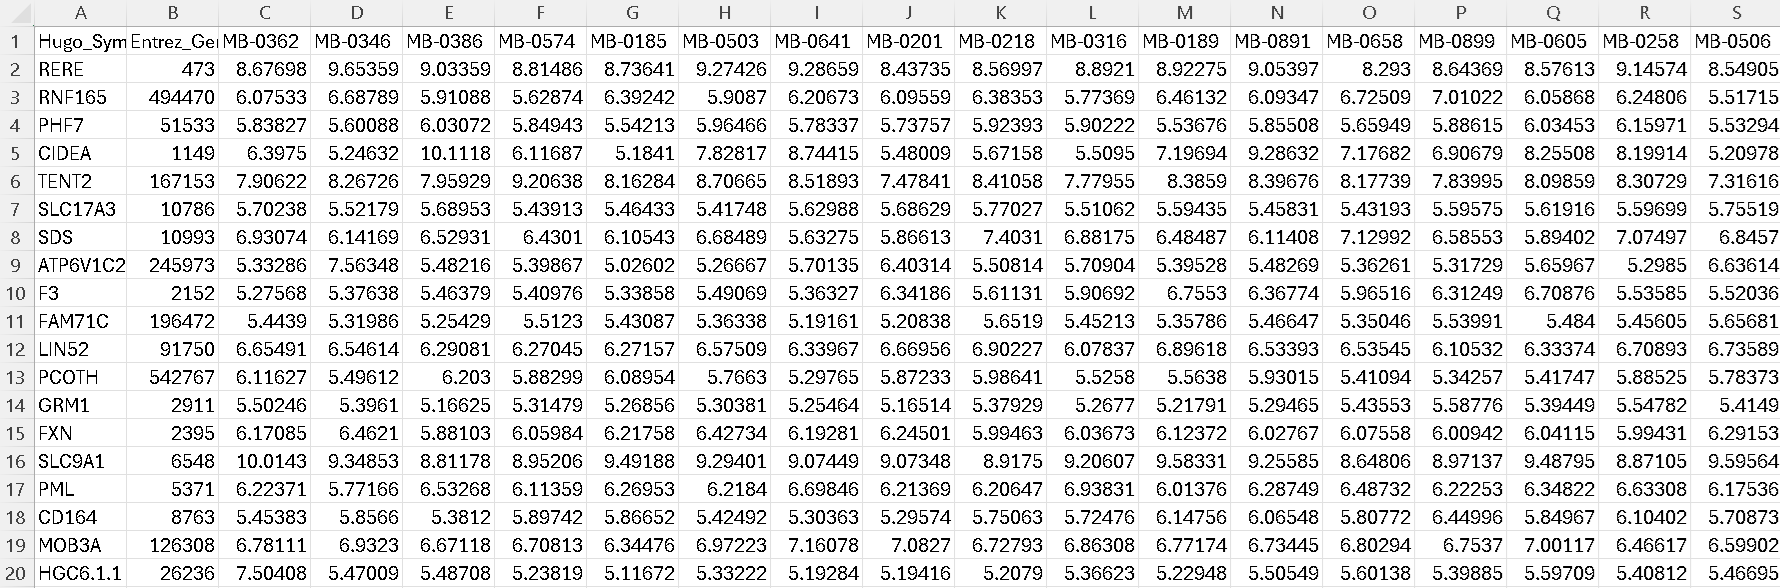
\includegraphics[width=\textwidth]{metabric_expr.png}
    \caption{METABRIC breast cancer gene expression dataset}
    \label{fig:metabric_expr}
\end{figure}

\begin{figure}[h!]
    \centering
    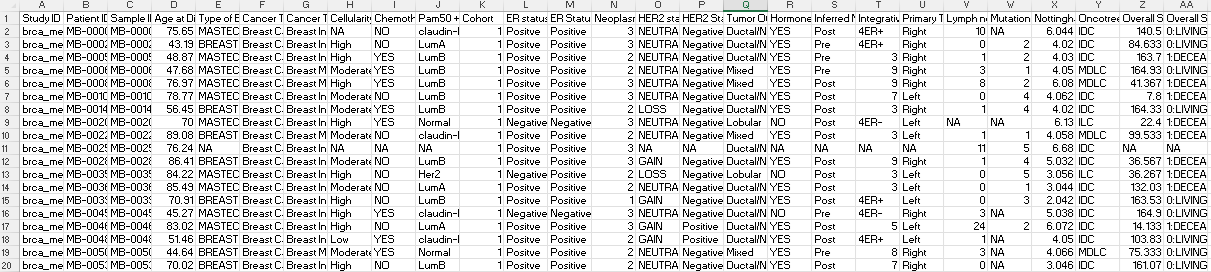
\includegraphics[width=\textwidth]{metabric_data.png}
    \caption{METABRIC breast cancer clinical data}
    \label{fig:metabric_data}
\end{figure}

\begin{figure}[h!]
    \centering
    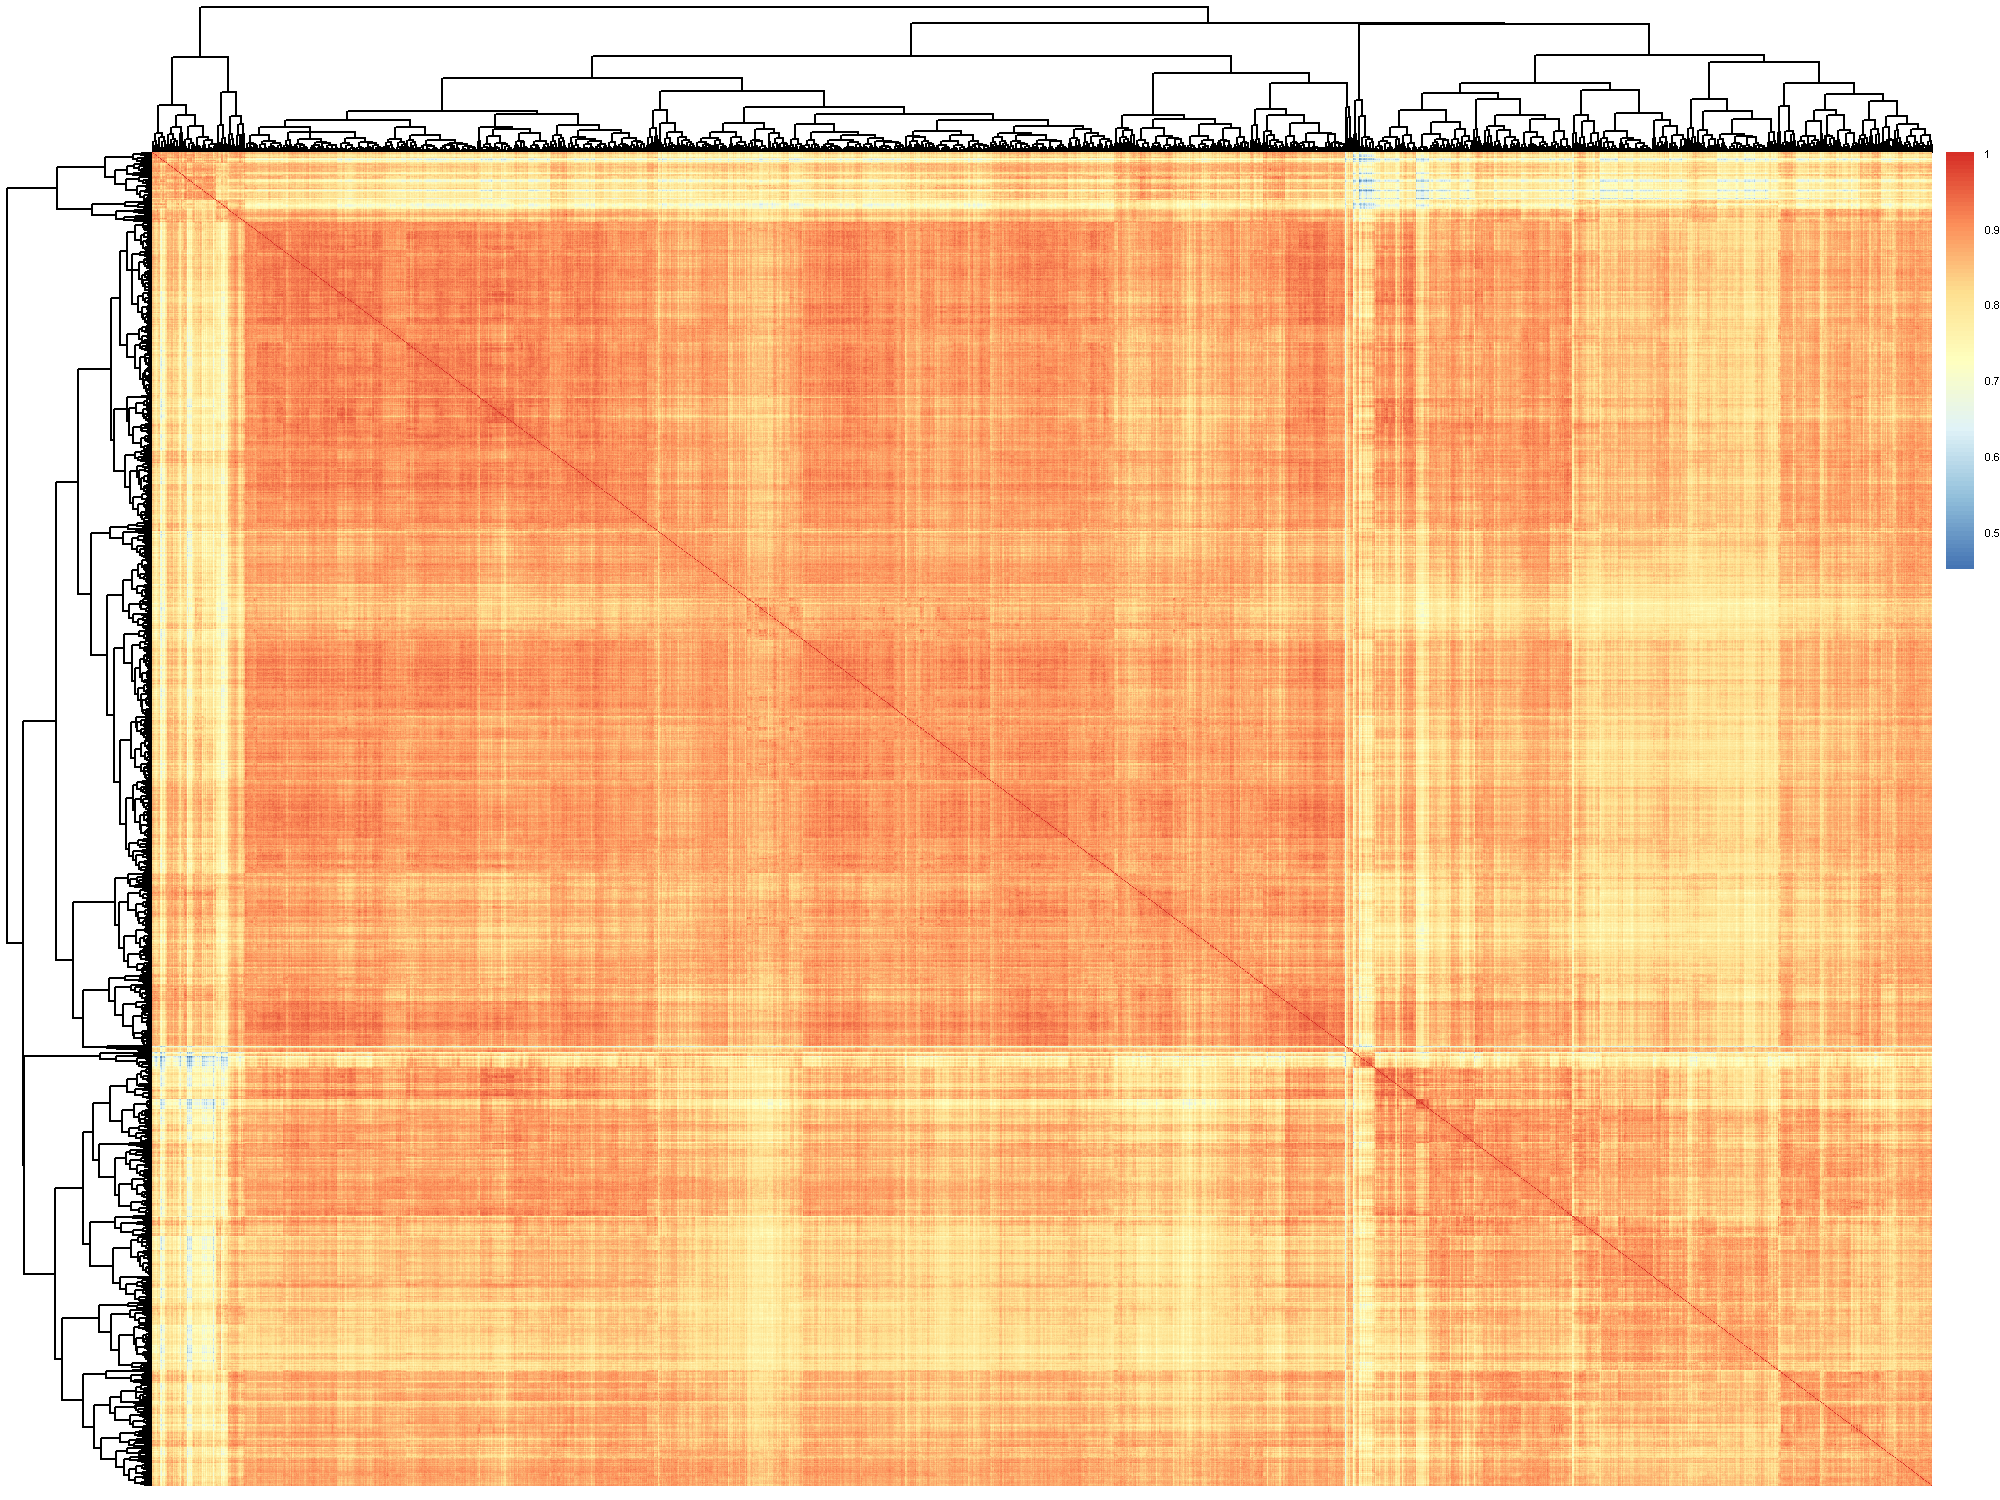
\includegraphics[width=0.8\textwidth]{metabric_corr.png}
    \caption{Correlation plot of METABRIC breast cancer gene expression dataset}
    \label{fig:metabric_corr}
\end{figure}

Alzheimer disease (AD) gene expression data~\citep{srinivasan2020alzheimer} contains 39,376 transcripts from post-mortem fusiform gyrus tissues of 289 AD subjects (see Fig.~\ref{fig:alzheimer_expr} for details). It also contained various clinical data for every sample, particularly the Braak stages of AD (see Fig.~\ref{fig:alzheimer_data} for details).

The Braak stages~\citep{braak1991neuropathological} describe how AD progresses in the brain, particularly on the spread of tau tangles. In Stage I, the tangles begin in the part of the brain responsible for memory. By Stage II, they spread to areas involved in memory processing. In Stage III, tangles reach regions related to both memory and emotions. As the disease advances to Stage IV, the tangles spread to more areas of the brain, leading to noticeable memory problems. In Stage V, tangles affect larger parts of the brain, and cognitive issues become more severe. Finally, in Stage VI, the tangles are widespread across the brain, and individuals experience severe dementia, with significant impairments in memory and cognition. As the Braak stages progress, the severity of memory and thinking problems increases.

\begin{figure}[h!]
    \centering
    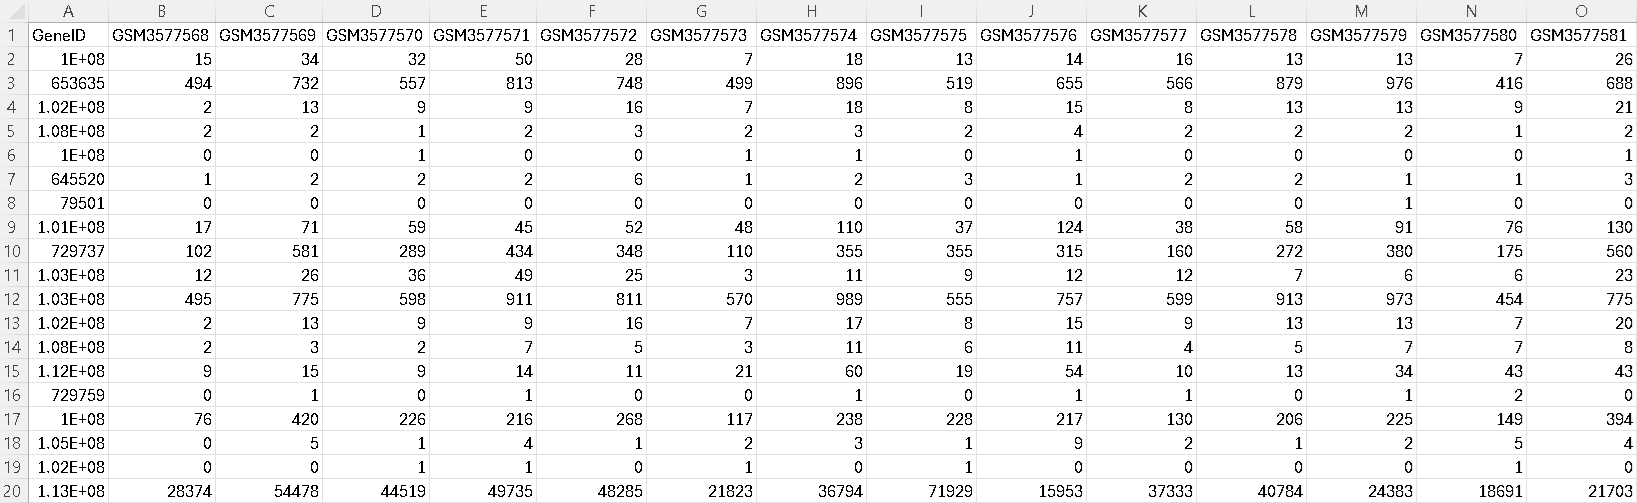
\includegraphics[width=\textwidth]{alzheimer_expr.png}
    \caption{Alzheimer disease gene expression dataset}
    \label{fig:alzheimer_expr}
\end{figure}

\begin{figure}[h!]
    \centering
    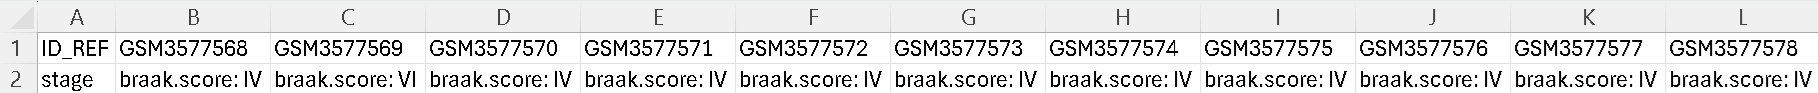
\includegraphics[width=\textwidth]{alzheimer_data.png}
    \caption{Alzheimer disease clinical data}
    \label{fig:alzheimer_data}
\end{figure}

\begin{figure}[h!]
    \centering
    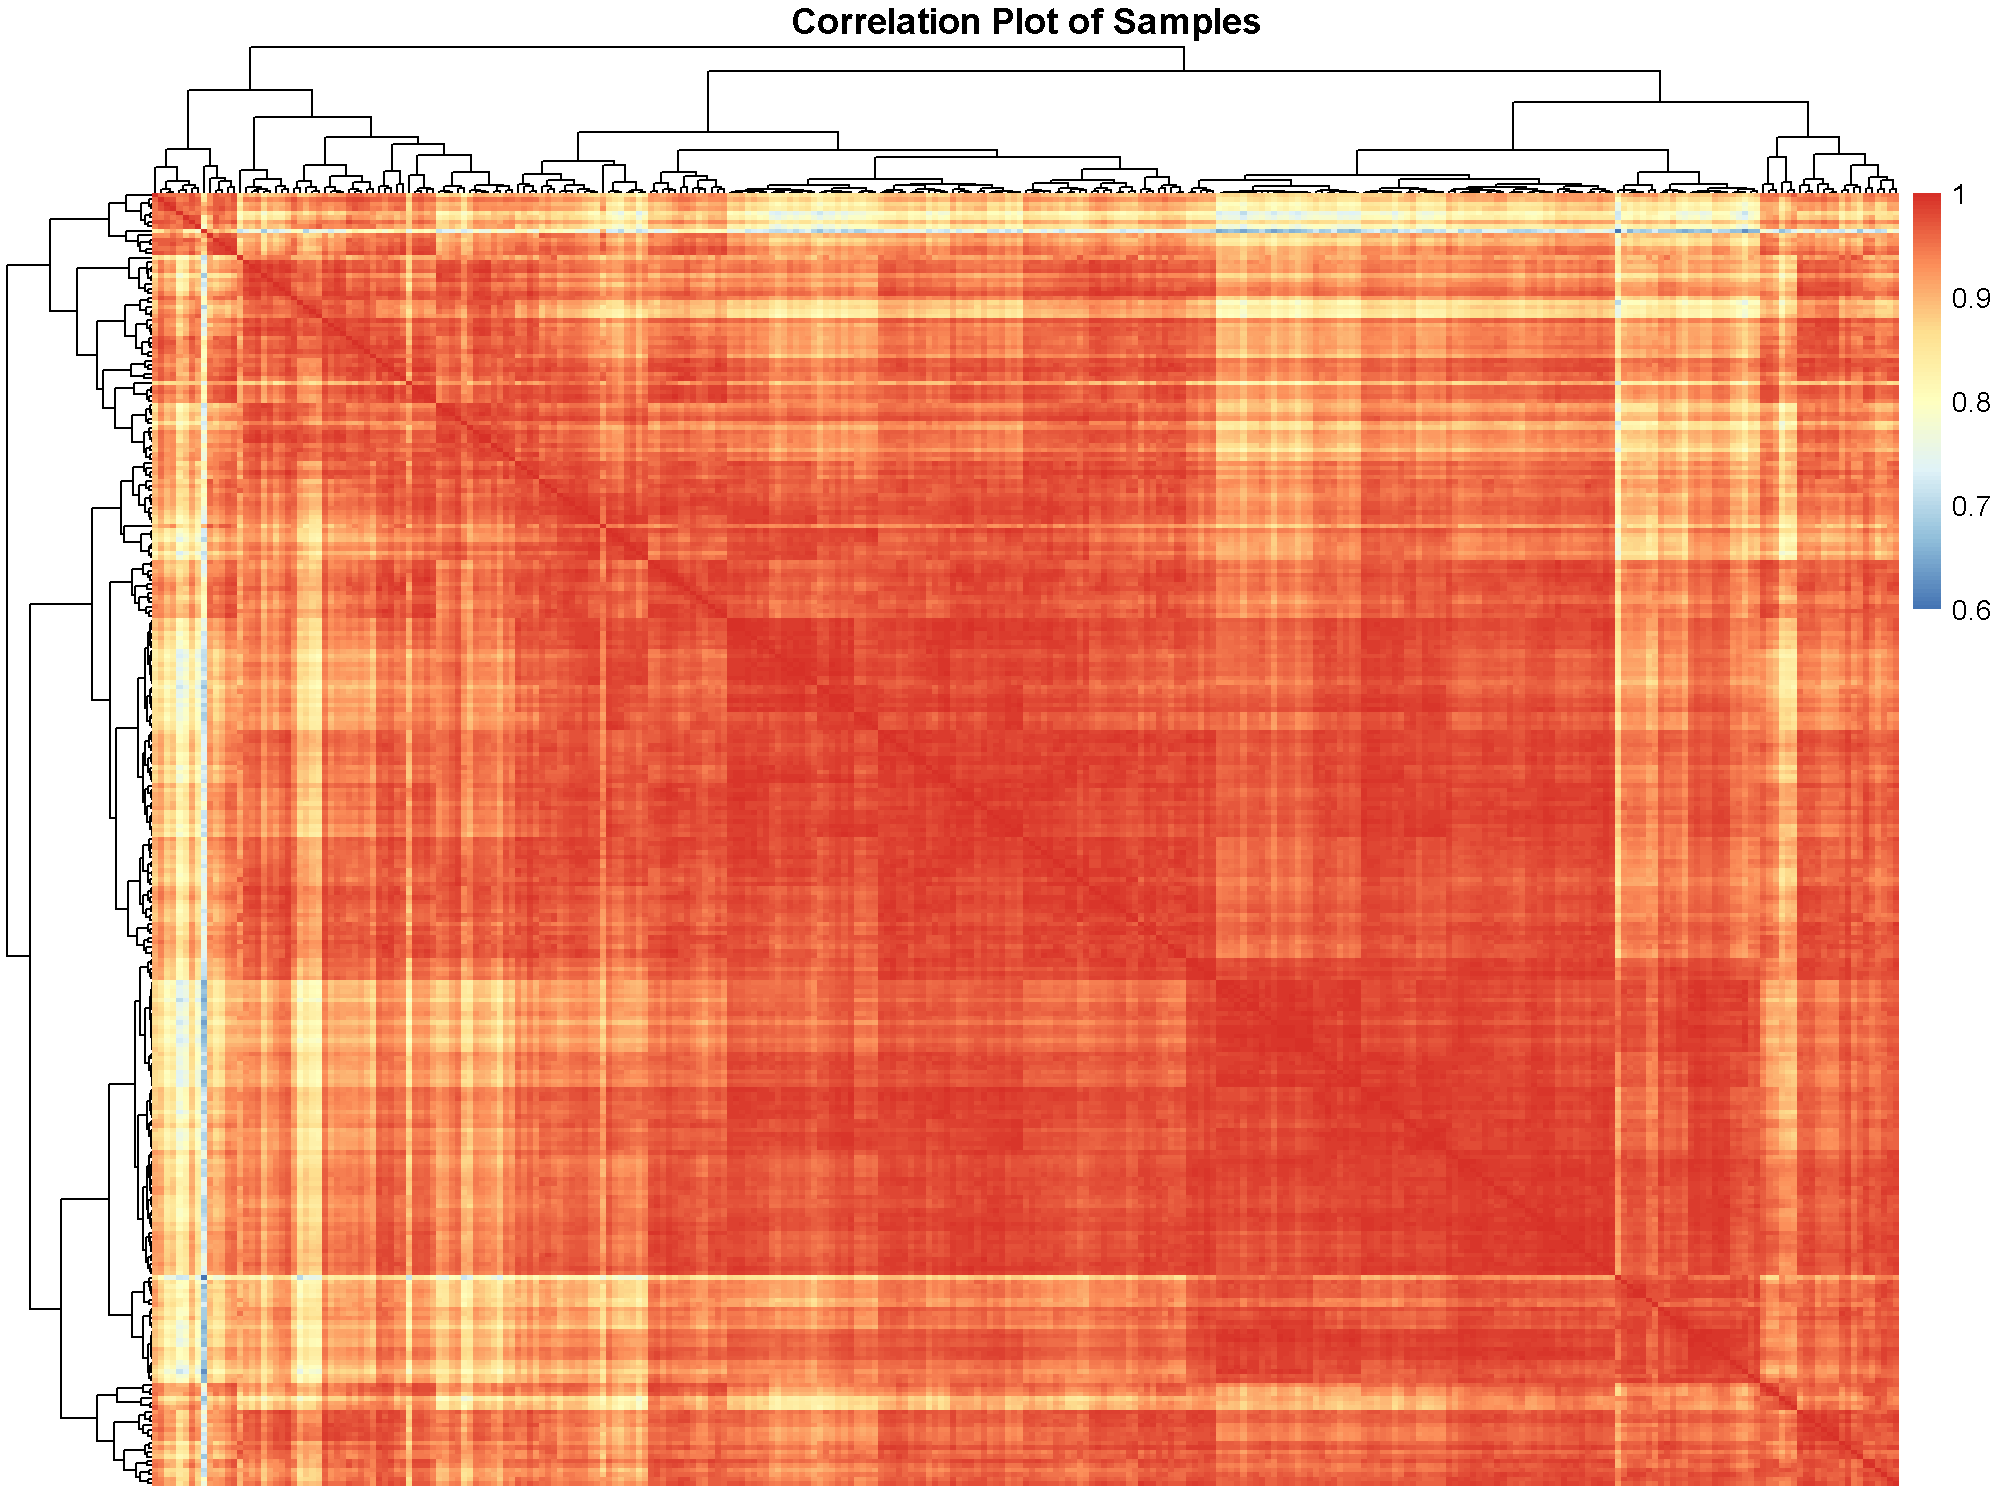
\includegraphics[width=0.8\textwidth]{alzheimer_corr.png}
    \caption{Correlation plot of Alzheimer disease gene expression dataset}
    \label{fig:alzheimer_corr}
\end{figure}

\section{Model and Methods Description}

The GuidedSparseK-means algorithm enhances traditional sparse K-means clustering by integrating clinical phenotypic data into the clustering process. The model employs a unified objective function that comprises three key components: a weighted K-means approach for effective sample clustering, lasso regularization for gene selection from high-dimensional omics data, and the incorporation of a phenotypic variable to guide the clustering towards biologically meaningful outcomes. This iterative optimization process simultaneously refines both sample clustering and gene selection, allowing the algorithm to uncover subtypes that are not only statistically robust but also aligned with clinical relevance. Through simulations and applications to real-world datasets, the performance of GuidedSparseK-means is benchmarked against existing clustering methods, demonstrating its superiority in capturing the complex relationships inherent in the data.

\subsection{K-means Algorithm}

The first clustering method the paper described is the normal k means algorithm. It considers $X_{gi}$ to be the gene expression of gene g and subject i. Let the total number of genes be G and the total number of subjects be n. The normal k means algorithm finds K clusters of our n subjects such that the clusters are close together (usually in the euclidean distance). Denote such an optimal clustering as $\hat{C}$. This is done by minimizing the objective function 
\begin{equation}
    \hat{C} = \textrm{argmin}_C \sum_{g=1}^G WCCS_g = \textrm{argmin}_C \sum_{g=1}^G \sum_{k = 1}^K \frac{1}{n_k} \sum_{(i,j) \in C_k} (X_{gi} - X_{gj})^2. 
\end{equation}
Where C is a partition of our data set into K clusters and $C_k$ for $1\leq k \leq K$ is the elements in the kth cluster and $n_k$ is the size of cluster k.

\subsection{Sparse K-means Algorithm}

Due to the nature of genetics data, we have that there are usually a significantly more number of genes than we have subjects. Thus, there is usually an assumption of sparsity in the number of genes that would actually have a significant impact on the clustering of subjects. The solution to taking into account this sparsity into our clustering is to maximize the weighted between cluster sum of squares subject to a LASSO like penalty. This usage of between cluster sum of squares is to avoid the issue of a trivial solution to equation (1) from a naive implementation of a lasso penalty. The sparse K means clustering, denoted as $\hat{C}_{Sparse}$, is found by maxizing the objective function 
\begin{equation}
    \hat{C}_{Sparse} = \textrm{argmax}_{C,w} w_g\left[\frac{1}{n} \sum_{i,j \in C} (X_{gi} - X_{gj})^2 - \sum_{k=1}^K \frac{1}{n_k}\sum_{i,j \in C_k} (X_{gi} - X_{gj})^2 \right]
\end{equation}
subject to $||w||_2 \leq 1$, $||w||_1 \leq s$, $w \geq 0$ and the weight vector discarded from the argmax. Above, we have that $s$ is a tuning parameter in order to control the number of genes we select. The $L_1$ penalty is chosen to cause gene selection and the $L_2$ penalty is additionally used to facilitate selecting more than one gene. Notice that the total sum of squares term is constant for all clusters and our problem thus involves minimizing the within cluster sum of squares with the additional weights.
    

\subsection{GuidedSparseKMeans}

The main novelty that this paper introduces is the addition of a guided term to our objective function for sprase k means. This is motivated by a desire to include information that we have from clinical outcomes into our clustering. We denote the association between a gene g and a given clinical outcome variable as $U_g$. In general the $U_g$ is defined in terms of a function $U: \RR^n \times \RR^n \rightarrow \RR$ such that $U_g = U(x_g, y)$, where $x_g$ is the expression level of gene g across all subjects and y is the vector of clinical outcomes. From above, we can see that $BCSS_g(C) = \left[\frac{1}{n} \sum_{i,j \in C} (X_{gi} - X_{gj})^2 - \sum_{k=1}^K \frac{1}{n_k}\sum_{i,j \in C_k} (X_{gi} - X_{gj})^2 \right]$ and $TSS_g = \frac{1}{n} \sum_{i,j \in C} (X_{gi} - X_{gj})^2$. With these, we can define our objective function fo the GuidedSparseKmeans with the optimal clustering being $\hat{C}_{GSK}$

\begin{equation}
    \hat{C}_{GSK} = \textrm{argmax}_{C,w} \sum_{g=1}^G w_g \left[ \frac{BCSS_g(C)}{TSS_g} + \lambda U_g  \right]
\end{equation}
subject to the constraints $||w||_2 \leq 1$, $||w||_1 \leq s$, $w \geq 0$. Similarly to above, the weight vector component of the argmax is discarded. Further, $\lambda$ is a tuning parameter to control how much of the clustering is guided by the clinical outcome and how much is guided by how much gene g affects the clustering separation. Notice further that the term corresponding to gene g separation ability is normalized by $TSS_g$ to allow this term to be comparable with the scale of $U_g$.  In the paper, the author chose to choose a $U_g$ such that it is based on a regression model $f_g$ which is univariate. Namely $y = f_g(x_g) + \varepsilon$ with $\varepsilon$ some error is the relationship between outcomes and gene expression. They defined $U_g$ such that it is the pseudo R-squared of this regression function. Namely,

\begin{equation*}
    U_g = 1- \left[\frac{L(f_0)}{L(f_g)} \right]^{2/n},
\end{equation*}

where $L(f_0)$ is the likelihood of the null model and $L(f_g)$ is the likelihood of the $f_g$ model. The GuidedSparseKMeans is computed in Algorithm 1. 

\begin{algorithm}
    \caption{GuidedSparseKmeans Algorithm}
    \begin{algorithmic}[1]
        \REQUIRE Number of clusters K, $\lambda$, s
        \INPUT Number of subjects n, number of subjects G, Gene data $X \in \RR^{n\times G}$, clinical outcome $U_g$
        \OUTPUT Optimal clustering $\hat{C}_{GSK}$ for GuidedSparseKmeans
        \STATE \textbf{Initialization} Let $U_g^* = U_g I(U_g \geq U_{(r)})$, where $U_{(r)}$ is the rth largest value of $U_j$ for $j = 1,\ldots, G$ (r = 400 was chosen for most of the implementation by the author). Initialize $w_g = \frac{U_g^*}{\sum_{g=1}^G U_g^*} \times s$
        \STATE Fix w and update $C_k$ with weighted K means. Namely we have $C(w) = \arg \max_C \sum_{g=1}^G w_g BCSS_g(C)$. 
        \STATE With C fixed, update w as $w_g(C) = \frac{S(a_g, b)}{||S||_2}$, wehre $S(x,c) = max(x-c, 0)$, $a_g = \frac{BCSS_g(C)}{TSS_g} + \lambda U_g$ where b is chosen such that the update weight vector as $L_1$ norm of s and $b=0$ is $||w||_1 \leq s$ and $S := (S(a_1,b), \ldots S(a_G, b)) \in \RR^G$. 
        \STATE Iterate the previous steps 2 and 3 until $\frac{||w^t - w^{t-1}||_1}{||w^{t-1}||_1} \leq 10^{-4}$ with t being the number of iterations and $w^t$ being the weight on the t-th iteration   
    \end{algorithmic}
\end{algorithm}


\section{Simulation Studies}

The data that was used for the simulation studies was outlined in the paper to best emulate certain characteristics of genetic data. There were 3 subtypes in this example, and the data was simulated to have intrinsic genes, confounding genes and noise genes that have a correlated structure. The ways to generate the 3 types of data are described in algorithm 2. 

\begin{algorithm}
    \caption{Gene Data Generation}
    \begin{algorithmic}[1]
        \INPUT Number of subtypes K, number of gene modules M
        \OUTPUT A data matrix $X$ containing the simulated gene data and a data vector Y containing clinical response
        \STATE \textbf{Initialization} K = 3, M = 20
        \STATE Simulate the number of subjects in each subtype $N_k \sim POI(100)$ for $1 \leq k \leq K$. The total number of subjects we have is thus $N = \sum_{k=1}^K N_k$
        \STATE Simulate M gene modules letting $n_m \sim POI(20)$, where $n_m$ is the number of features in module m.
        \STATE Let $\theta_k$ be baseline expression of the gene of subtype k and $\theta_k = 2 + 2k$. $\mu_{km}$ is the template gene expression of subtype k and module m. We let $\mu_{km} = \alpha_m\theta_k + Z$ with $\alpha_m \sim UNIF((-2,-0.2 \cup (0.2,2))$, where $Z \sim N(0,1)$.
        \STATE Generate $X_{kmi}' \sim N(\mu_{km}, 9)$, where 9 is the biological variation in the gene expression. 
        \STATE Sample $\Sigma_{km}' \sim W^{-1}(\phi, 60)$, where $\phi = 0.5 I_{n_m \times n_m} + 0.5*1_{n_m\times n_m}$, where $1_{x\times y}$ is the $x\times y$ dimensional matrix with elements of all 1.
        \STATE Calculate gene covariance matrix for sutype k and module m $\Sigma_{km}$ by standardizing $\Sigma_{km}'$ such that the diagonal is all 1.
        \STATE Intrinsic Gene expression data for subject i in subtype k and module m is $(X_{1kmi}, \ldots, X_{n_mkmi})^T \sim MVN(X_{kmi}', \Sigma_{km})$
        \STATE Parition your N total subjects randomly into 3 groups.
        \STATE Generate expression data as in steps 3-8 using another 20 modules.
        \STATE Repeat steps 9-10 3 more times to get confounding gene expression data
        \STATE Generate 8000 noise genes with $\mu_g \sim Unif(4,8)$ and $X_{gi} \sim N(\mu_g, 1)$
        \STATE Simulate clinical response for subject i in subclass k with $Y_{ik} \sim N(\theta_k, 64)$.
    \end{algorithmic}
\end{algorithm}

\section{Application to Alzheimer’s Disease Data-Results}

This section describes the application of sparse K-means and GuidedSparseKmeans to an RNA-seq dataset from Alzheimer’s disease (AD) patients. AD is a severe neurodegenerative disorder that affects older adults. Its key features include neurofibrillary tangles and neuritic plaques. The dataset consisted of 30,727 transcripts from post-mortem fusiform gyrus tissues of 217 individuals. It is available publicly under GEO ID GSE125583. The data was processed by normalizing gene expression values, filtering out the 50\% lowest-expressed genes, and standardizing each gene to have a mean of 0 and a standard deviation of 1. This resulted in 15,363 genes used for further analysis.

The Braak stage was selected as the clinical outcome variable. It is a measure of the severity of neurofibrillary tangles and is widely used in AD research. Since the Braak stage includes six levels (1 to 6), we treated it as a continuous variable. We calculated $U_g$, the $R^2$ value, from univariate linear regression between each gene and the Braak stage. The number of clusters ($K$) was set to six, matching the six Braak stages. We used the method described above to automatically select the tuning parameter $\lambda$. The parameter $s$ was set to select 396 genes, close to the target of 400 genes. The GuidedSparseKmeans algorithm completed the analysis in 7 seconds, while sparse K-means required 22 seconds.

Heatmaps of the selected genes from both methods showed a gradient in expression levels. Expression ranged from low (green) to high (red). Clusters were labeled 1 to 6 to reflect these levels. We evaluated the biological relevance of the AD subtypes by calculating Pearson correlation coefficients between the cluster labels and Braak stages. The GuidedSparseKmeans clusters had a higher correlation (0.282) compared to those from sparse K-means (0.056). This suggests that the subtypes identified by GuidedSparseKmeans were more strongly linked to neurofibrillary tangles.

We also assessed how well the clusters from GuidedSparseKmeans reflected Braak stage information. The relevancy score was high ($Rel = 0.309$), confirming that the algorithm effectively utilized the clinical outcome variable. Pathway enrichment analysis further supported the biological significance of the selected genes. Using the BioCarta database, we found that the genes identified by GuidedSparseKmeans were enriched in the GPCR signaling pathway ($p = 6.59 \times 10^{-6}$) and the NOS1 signaling pathway ($p = 1.61 \times 10^{-5}$). Both pathways are known to play roles in AD. In contrast, sparse K-means did not identify these pathways.

In summary, GuidedSparseKmeans outperformed sparse K-means in identifying AD subtypes and selecting disease-relevant genes. Its ability to incorporate clinical guidance made it more effective in uncovering biologically meaningful insights.

\section{Discussion}
This paper introduces the outcome-guided sparse K-means algorithm, a novel approach for integrating clinical outcome data with high-dimensional omics data to identify meaningful disease subtypes. The algorithm addresses key challenges in statistical analysis, including gene selection from large datasets, the incorporation of various types of clinical outcome variables (e.g., continuous, binary, ordinal, or survival data), automatic tuning of parameters, and the evaluation of the relevance between the identified subtypes and the clinical outcomes. Its performance has been demonstrated through both simulations and real-world applications, including breast cancer and Alzheimer’s disease (AD), where it outperforms traditional sparse K-means methods.

A distinguishing feature of this algorithm is its use of clinical outcomes as guidance, ensuring that the resulting subtypes are both biologically interpretable and clinically relevant. For example, the Braak stage was selected as the guidance variable in the AD application due to its established role in measuring disease severity. Similarly, in breast cancer, HER2-guided clustering produced results with significant survival differences and biologically meaningful pathway analyses. In situations where domain knowledge is limited, the authors recommend testing multiple outcomes and selecting the one that yields the most interpretable clustering results. 

The algorithm’s parameters, including the number of clusters (K), penalty term ($\lambda$), and sparsity level (s), were estimated using gap statistics, sensitivity analysis, and extended gap statistics, respectively. While alternative methods for simultaneous parameter estimation exist, the authors highlight the need for further development of unified approaches. The robustness of the algorithm was evaluated under different scenarios, including varying numbers of selected genes and misspecification of the number of clusters. Simulations indicated that misspecifying K had a significant impact on clustering performance, whereas in real datasets, where cluster boundaries are gradual, the effects were less pronounced.

The computational efficiency of the algorithm is another significant strength. For example, the breast cancer dataset with over 12,000 genes and 1,870 samples required only 31 seconds to analyze. Similarly, the AD dataset with 15,000 genes and 217 samples was processed in just 7 seconds. The method has been implemented in the R package GuidedSparseKmeans, which is publicly available on GitHub.

\section{Conclusion}

The outcome-guided sparse K-means algorithm represents a significant advancement in the integration of clinical and omics data. It provides a reliable framework for identifying biologically and clinically meaningful subtypes of diseases. With the growing availability of comprehensive clinical and omics datasets, this method is expected to have broad applicability in understanding complex diseases.

The study by~\cite{meng2022outcome} demonstrated concrete evidence of the advantages of using the outcome-guided sparse K-means algorithm over other methods. They provided both simulation results and analyses from two real-world datasets to support their claims. However, several issues arose when attempting to replicate their results.

Firstly, the data we obtained using the link provided in the paper contained different numbers of genes and subjects than those reported. For instance, in their METABRIC example, they reported 24,368 genes and 1,981 subjects. However, the METABRIC data we obtained from their link contained only 20,603 genes and 2,501 subjects. Similarly, they stated that the Alzheimer’s dataset comprised 30,727 transcripts and 217 AD subjects. In contrast, the data we gathered contained 39,376 transcripts and 289 AD subjects.

Secondly, the details of data preprocessing were ambiguous, making it very challenging to arrive at the same final numbers of genes and subjects as reported in the paper. For example, in their motivating example section, they mentioned selecting 408 genes from the 12,180 genes in the METABRIC dataset as input for their algorithm. However, no explanation was provided regarding how these genes were selected.

Thirdly, the code they shared on GitHub was minimal, which made it very difficult for us to replicate their results. It would have been helpful if the code for generating each figure in the paper had been provided.

\section{Author Contribution Statement}

\textbf{I Hung:} Conceptualization, Investigation, Writing-Original draft preparation. \textbf{Nathan:} Conceptualization, Investigation, Methodology, Formal analysis, Writing-Original draft preparation. \textbf{Paul:} Conceptualization, Investigation, Data curation, Writing-Original draft preparation, Visualization, Validation.

\section{Citations and References}

\bibliography{reference}

\end{document}
